\chapter{Ongoing work and future directions}\label{chap:future}

There is still a lot that can be done to improve the detector in various fronts, this chapter suggests possible paths to build upon the work included in this document.

\section{Electronics}

Further finetuning of components needs to be done to ensure the best performance possible, the peak detectors's behavior has been found to be quite sensitive to the diode choices, so far it seems that the CMHSH-3 TR PBFREE schottky diode by Central Semiconductor Corp offers the best performance. In addition to this further exploration of amplifier and peak detector designs with different op-amp ICs may result extremely beneficial.

\subsection{Microcontroller}

\subsubsection{Code}

An interesting route yet to be explored is the use of the \texttt{C++} SDK, MicroPython has shown some limitations in speed, as showcased in subsection \ref{sec:ADC_shortcomings}, reducing the time delay in ADC readings could greatly improve resolution.

\subsubsection{Hardware}

As mentioned in subsection \ref{sec:ADC_shortcomings}, the Pico's ADC has shown some odd behaviors (seemingly low sensitivity every eight channels) which need to be further studied in order to improve the reliability of the measurement. On top of this, we are currently not taking full advantage of the 12-bit resolution in the ADC, since the peak detector gets saturated at around one Volt. The RP2040 documentation has some suggestions that could improve the ADC resolution \cite{datasheet2024RpPico} in our case, like removing the onboard resistor \textit{R7} to change the ADC voltage reference, which is set at 3.3 \unit{\V} by default, leaving 2.3 \unit{\V} unused due to our peak detector limitations.

\section{Geant4 simulation}

\subsection{Adding LYSO radioactivity}

As mentioned in Section \ref{sec:self_radiation} and subsection \ref{sec:simulated_spectra}, LYSO:Ce crystals have self radiation, this feature has not yet been added to the simulation and would be an interesting exercise to showcase how Geant4 can recreate this type of physical process.

\subsection{Improving data recollection}

All the results included in Chapter \ref{chap:G4_simulations} are extracted in \texttt{stepAction.cc}, by checking the current volume of the particle and extracting data accordingly. This approach, however, is very inefficient, since it performs multiple operations for every step of every particle created in the simulation. In order to improve this one could make use of the \texttt{G4VSensitiveDetector} class, which calls the \texttt{ProcessHits} function once a particle enters the sensitive volume, in our case this volume could be the SiPM or scintillating material. Additionally, the use of \texttt{ROOT} with binary files could be a great introduction for students to this tool data analysis tool, which is widely used in particle physics for data analysis.

\section{Odd features in measured spectra}

Figure \ref{fig:NIM_odd_features} showcases odd features found while measuring spectra with the NIM modules, some of which can also be found in the spectra obtained with the Rohde\&Schwarz oscilloscope. The high number of counts above the photopeak and the oddly shaped photopeaks (``shoulders'' on the high energy side, also discussed in \cite{peak_shoulders}) could make for an interesting study.

\section{Testing different scintillator sizes and materials}

\begin{figure}[H]
    \begin{subfigure}[t]{0.49\textwidth}
        \centering
        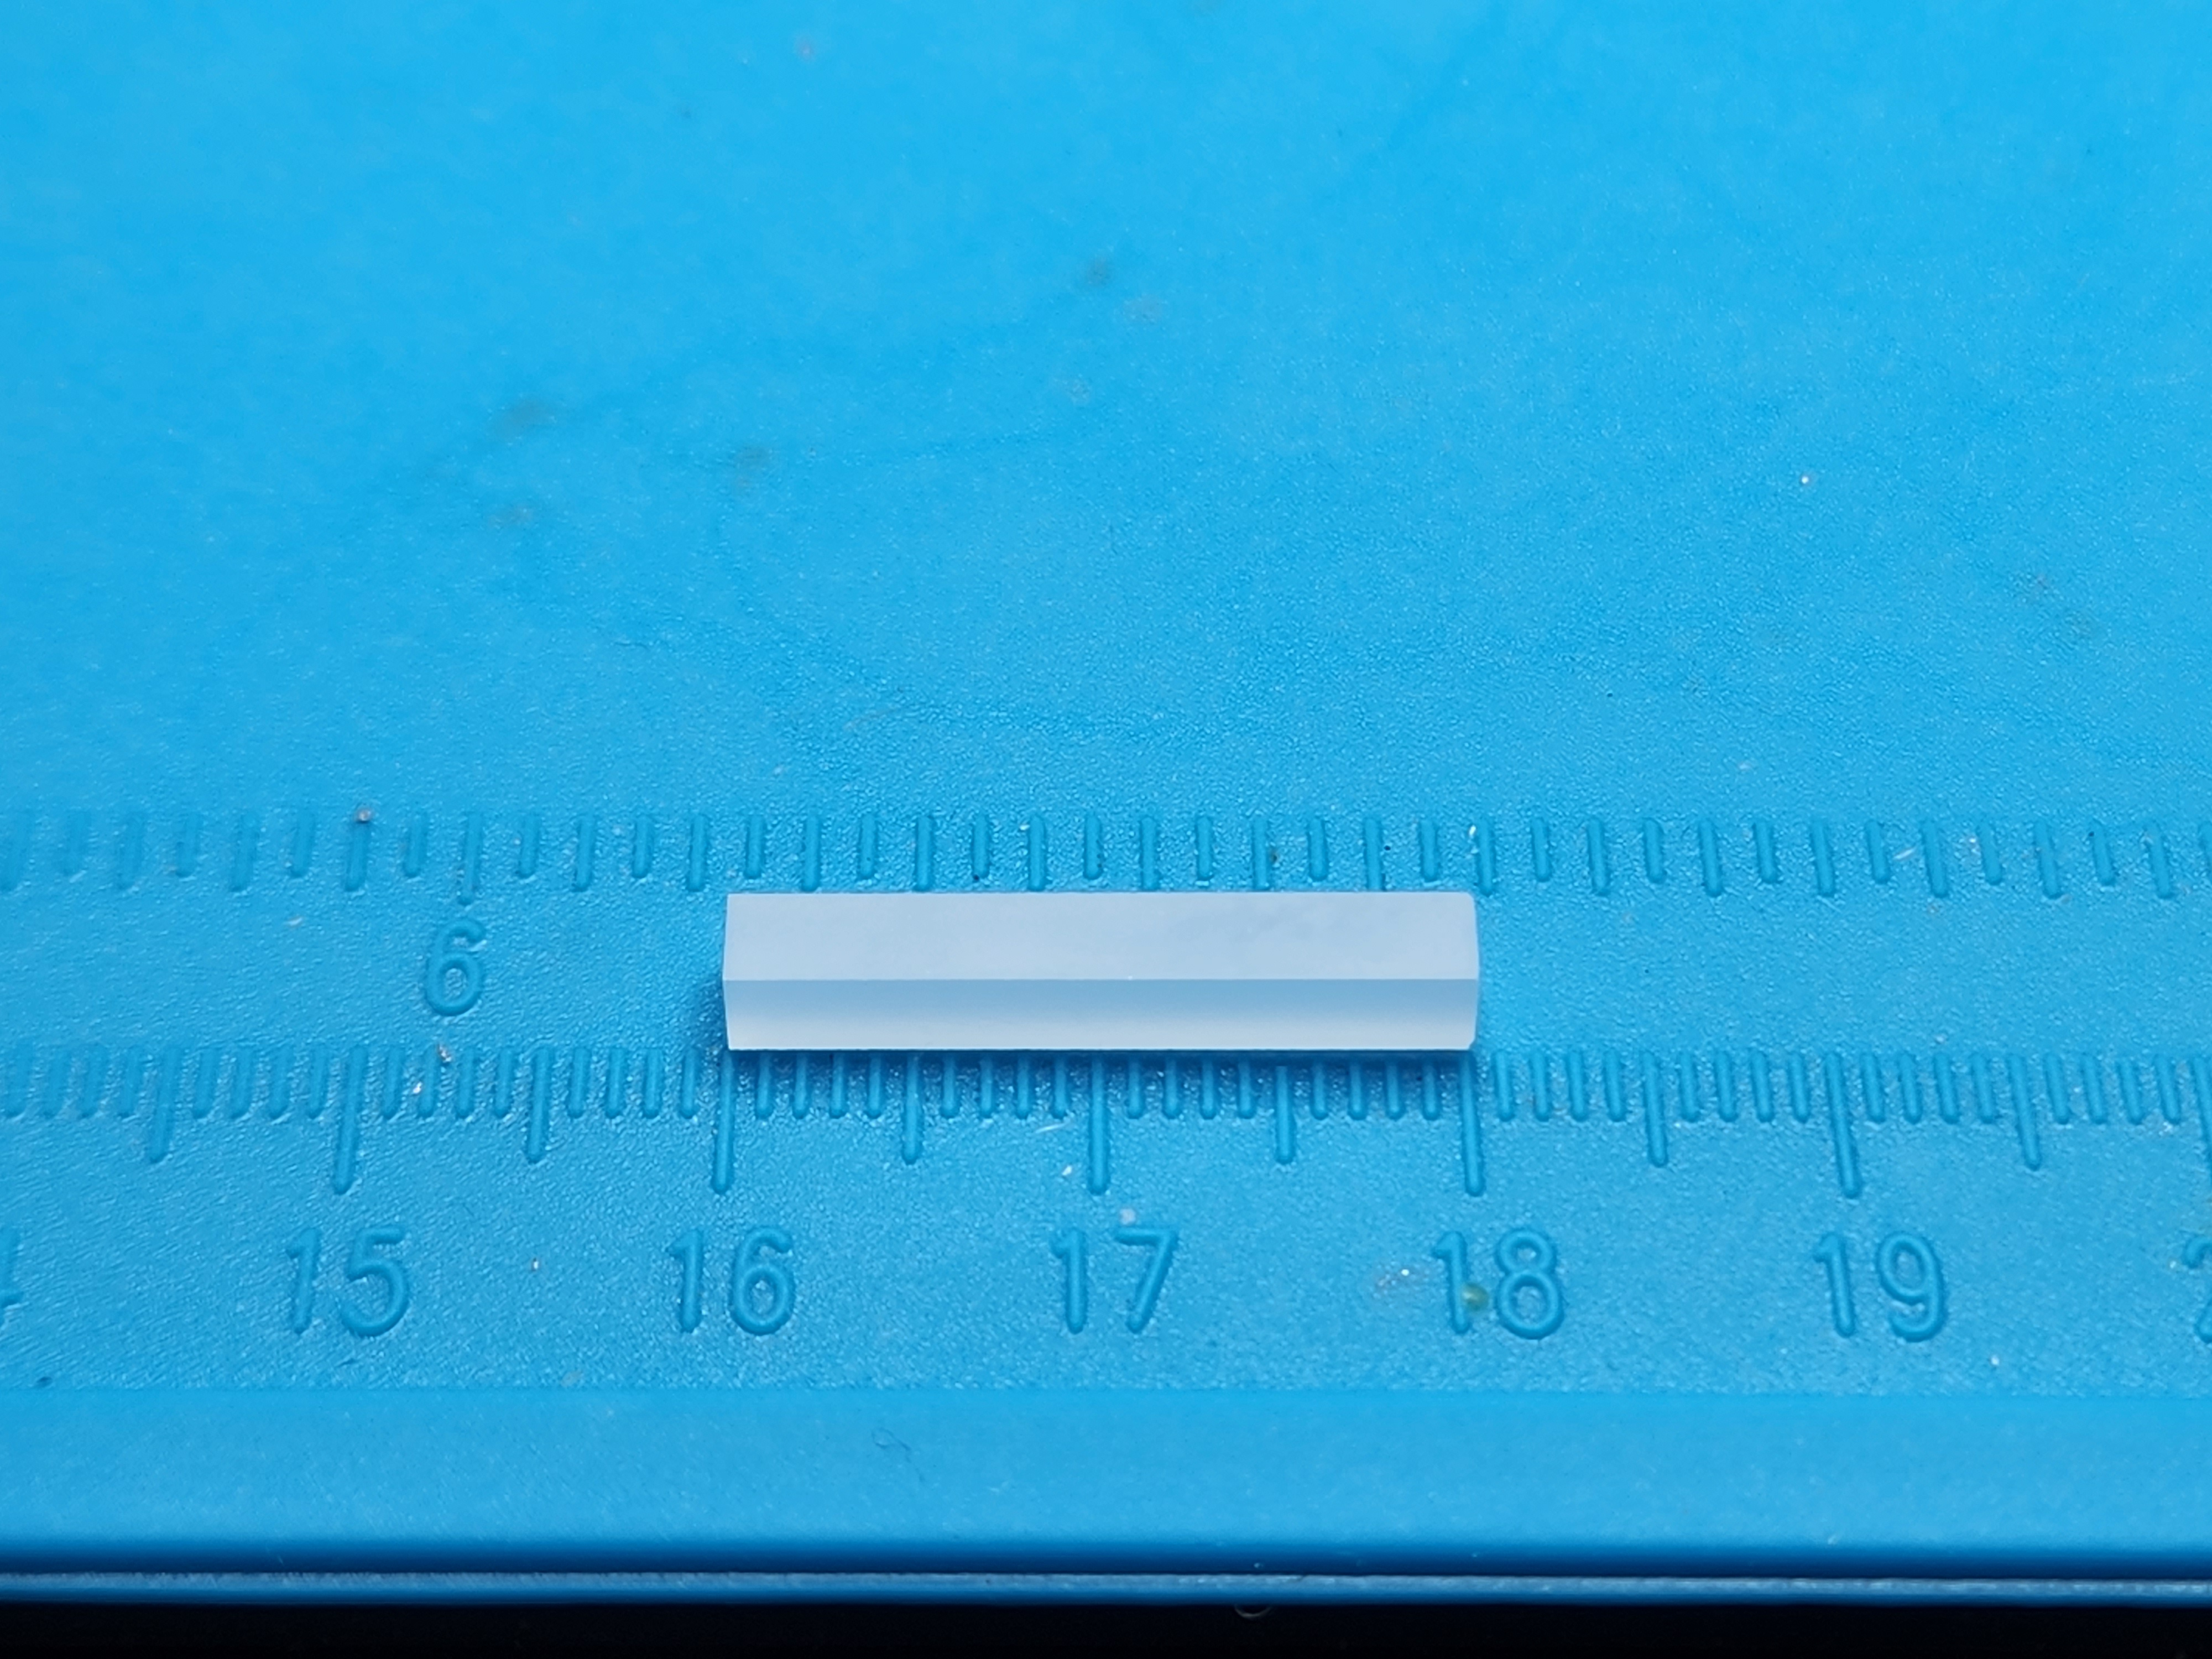
\includegraphics[width=.7\textwidth]{future/LYSO_crystals/LYSO_20_3_3.jpg}
    \end{subfigure}
    \begin{subfigure}[t]{0.49\textwidth}
        \centering
        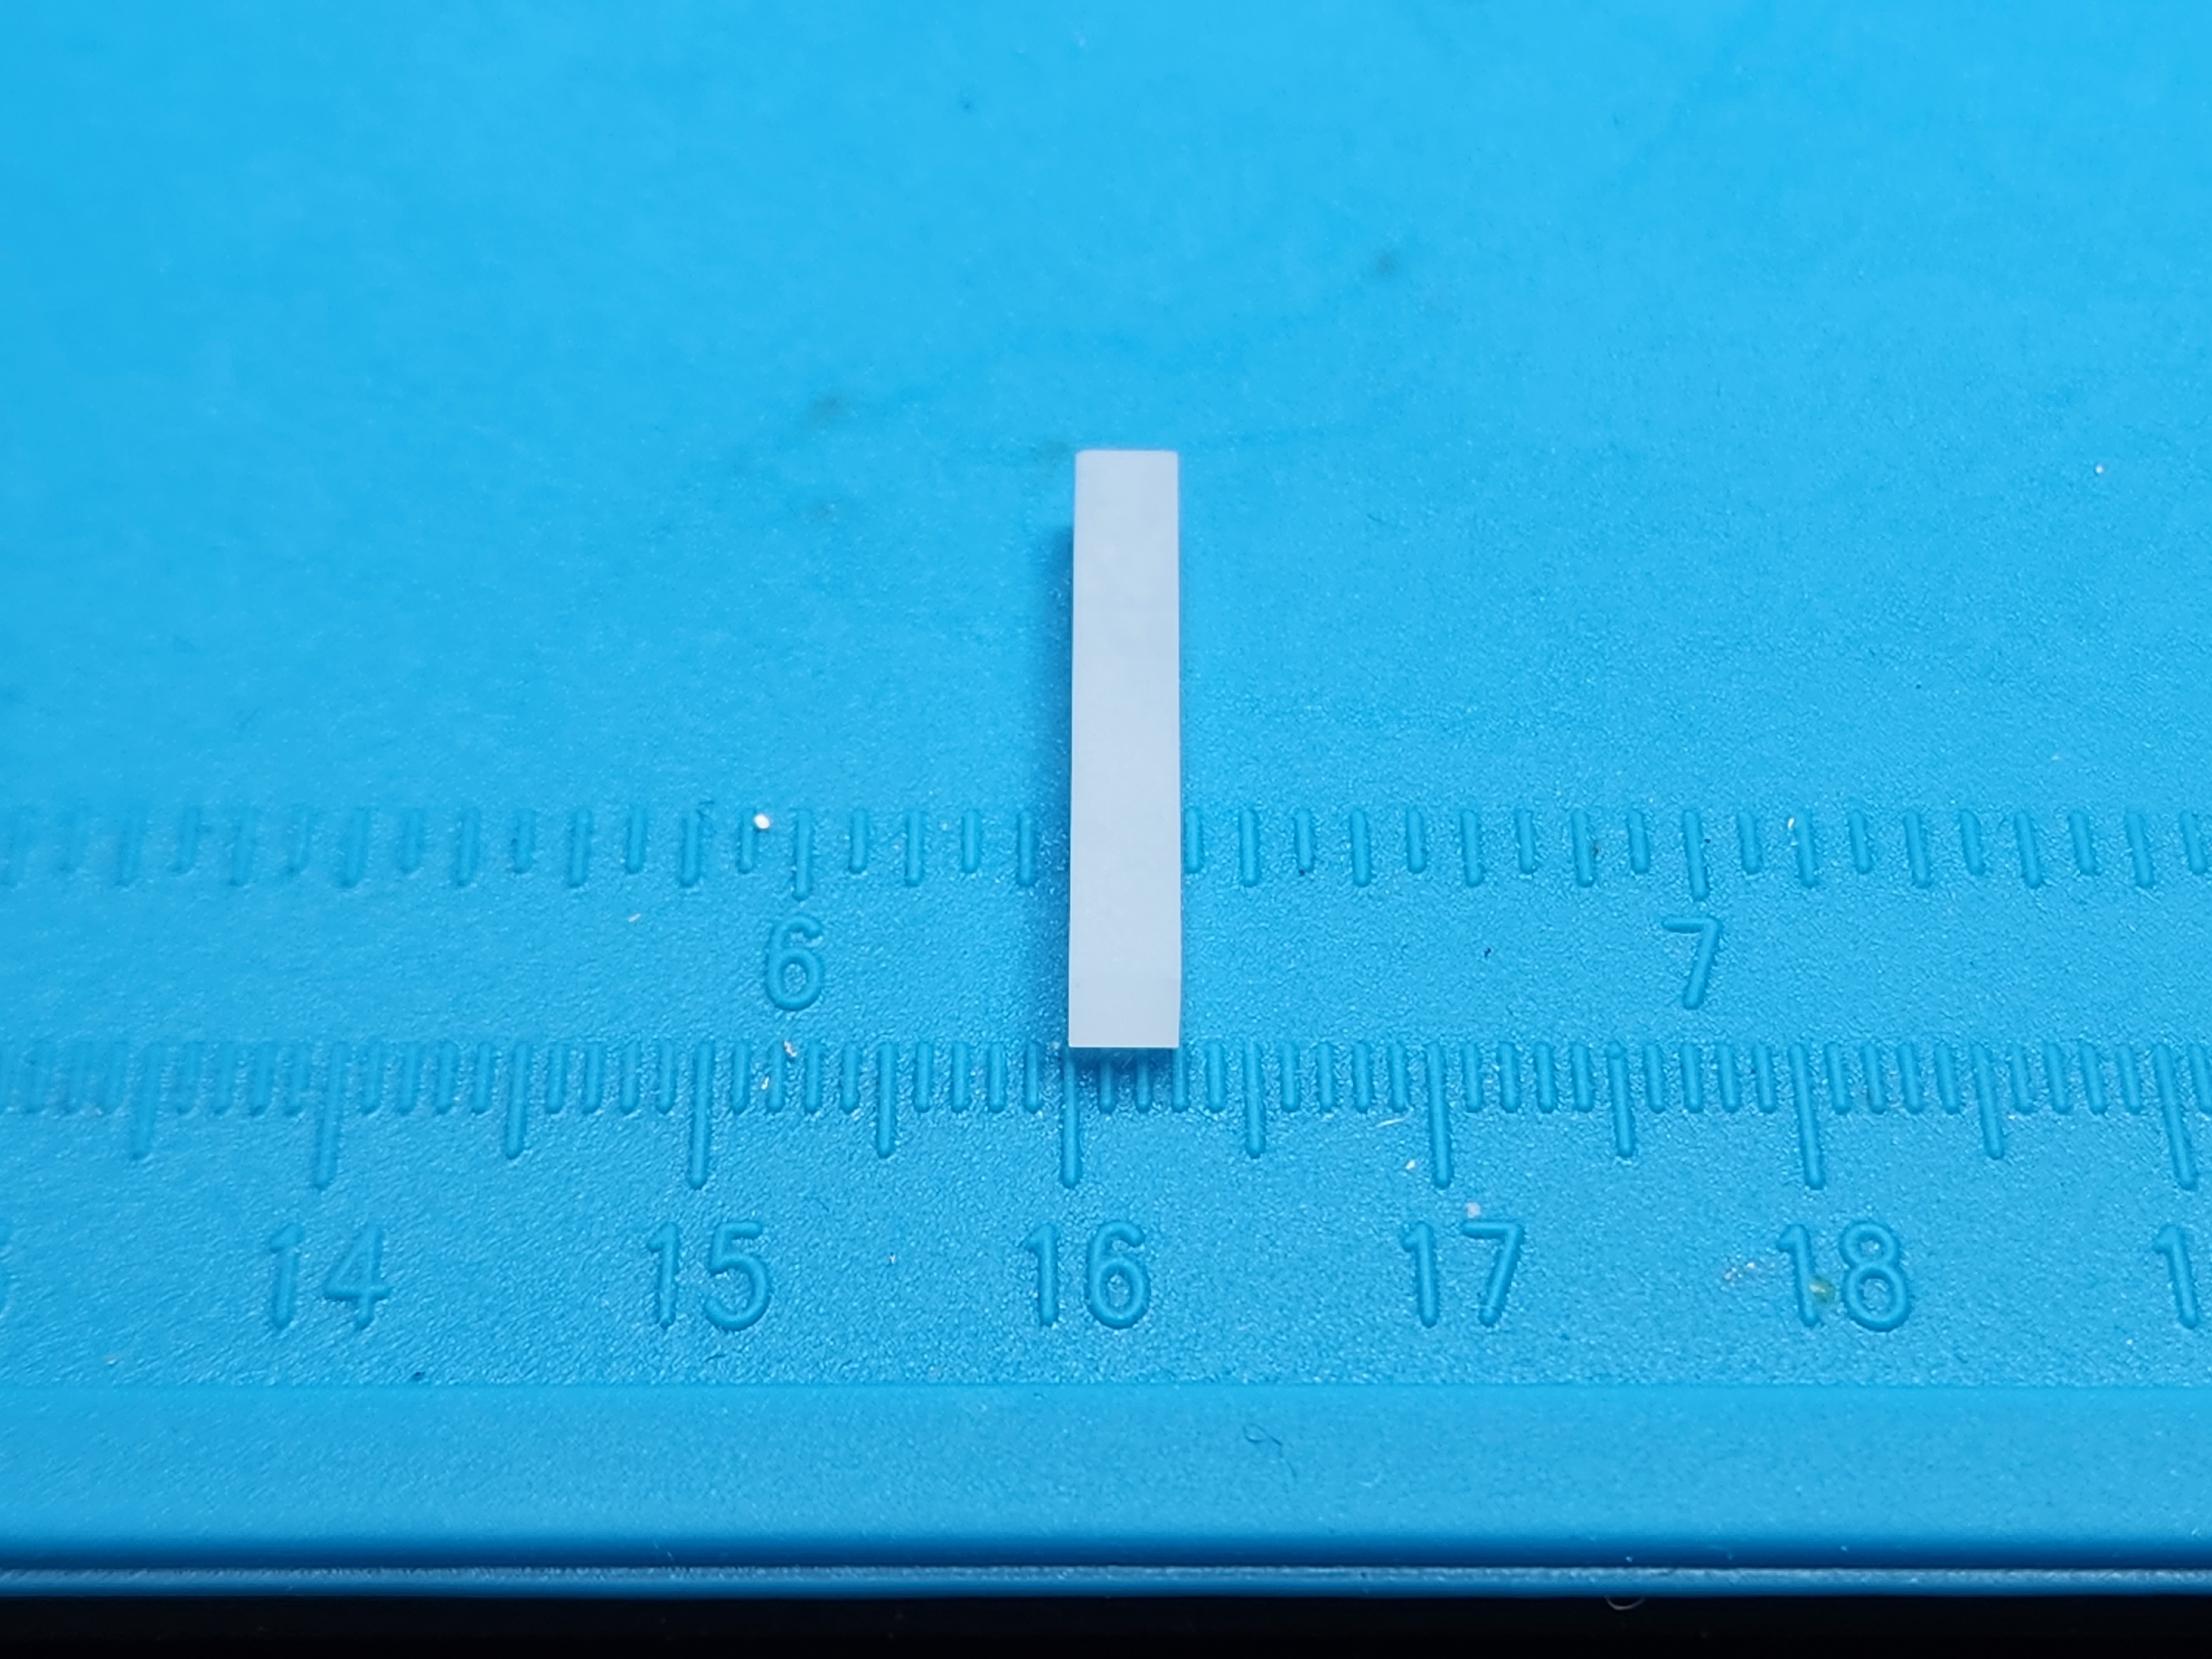
\includegraphics[width=.7\textwidth]{future/LYSO_crystals/LYSO_20_3_3_2.jpg}
    \end{subfigure}
    \medskip
    \begin{subfigure}[t]{0.49\textwidth}
        \centering
        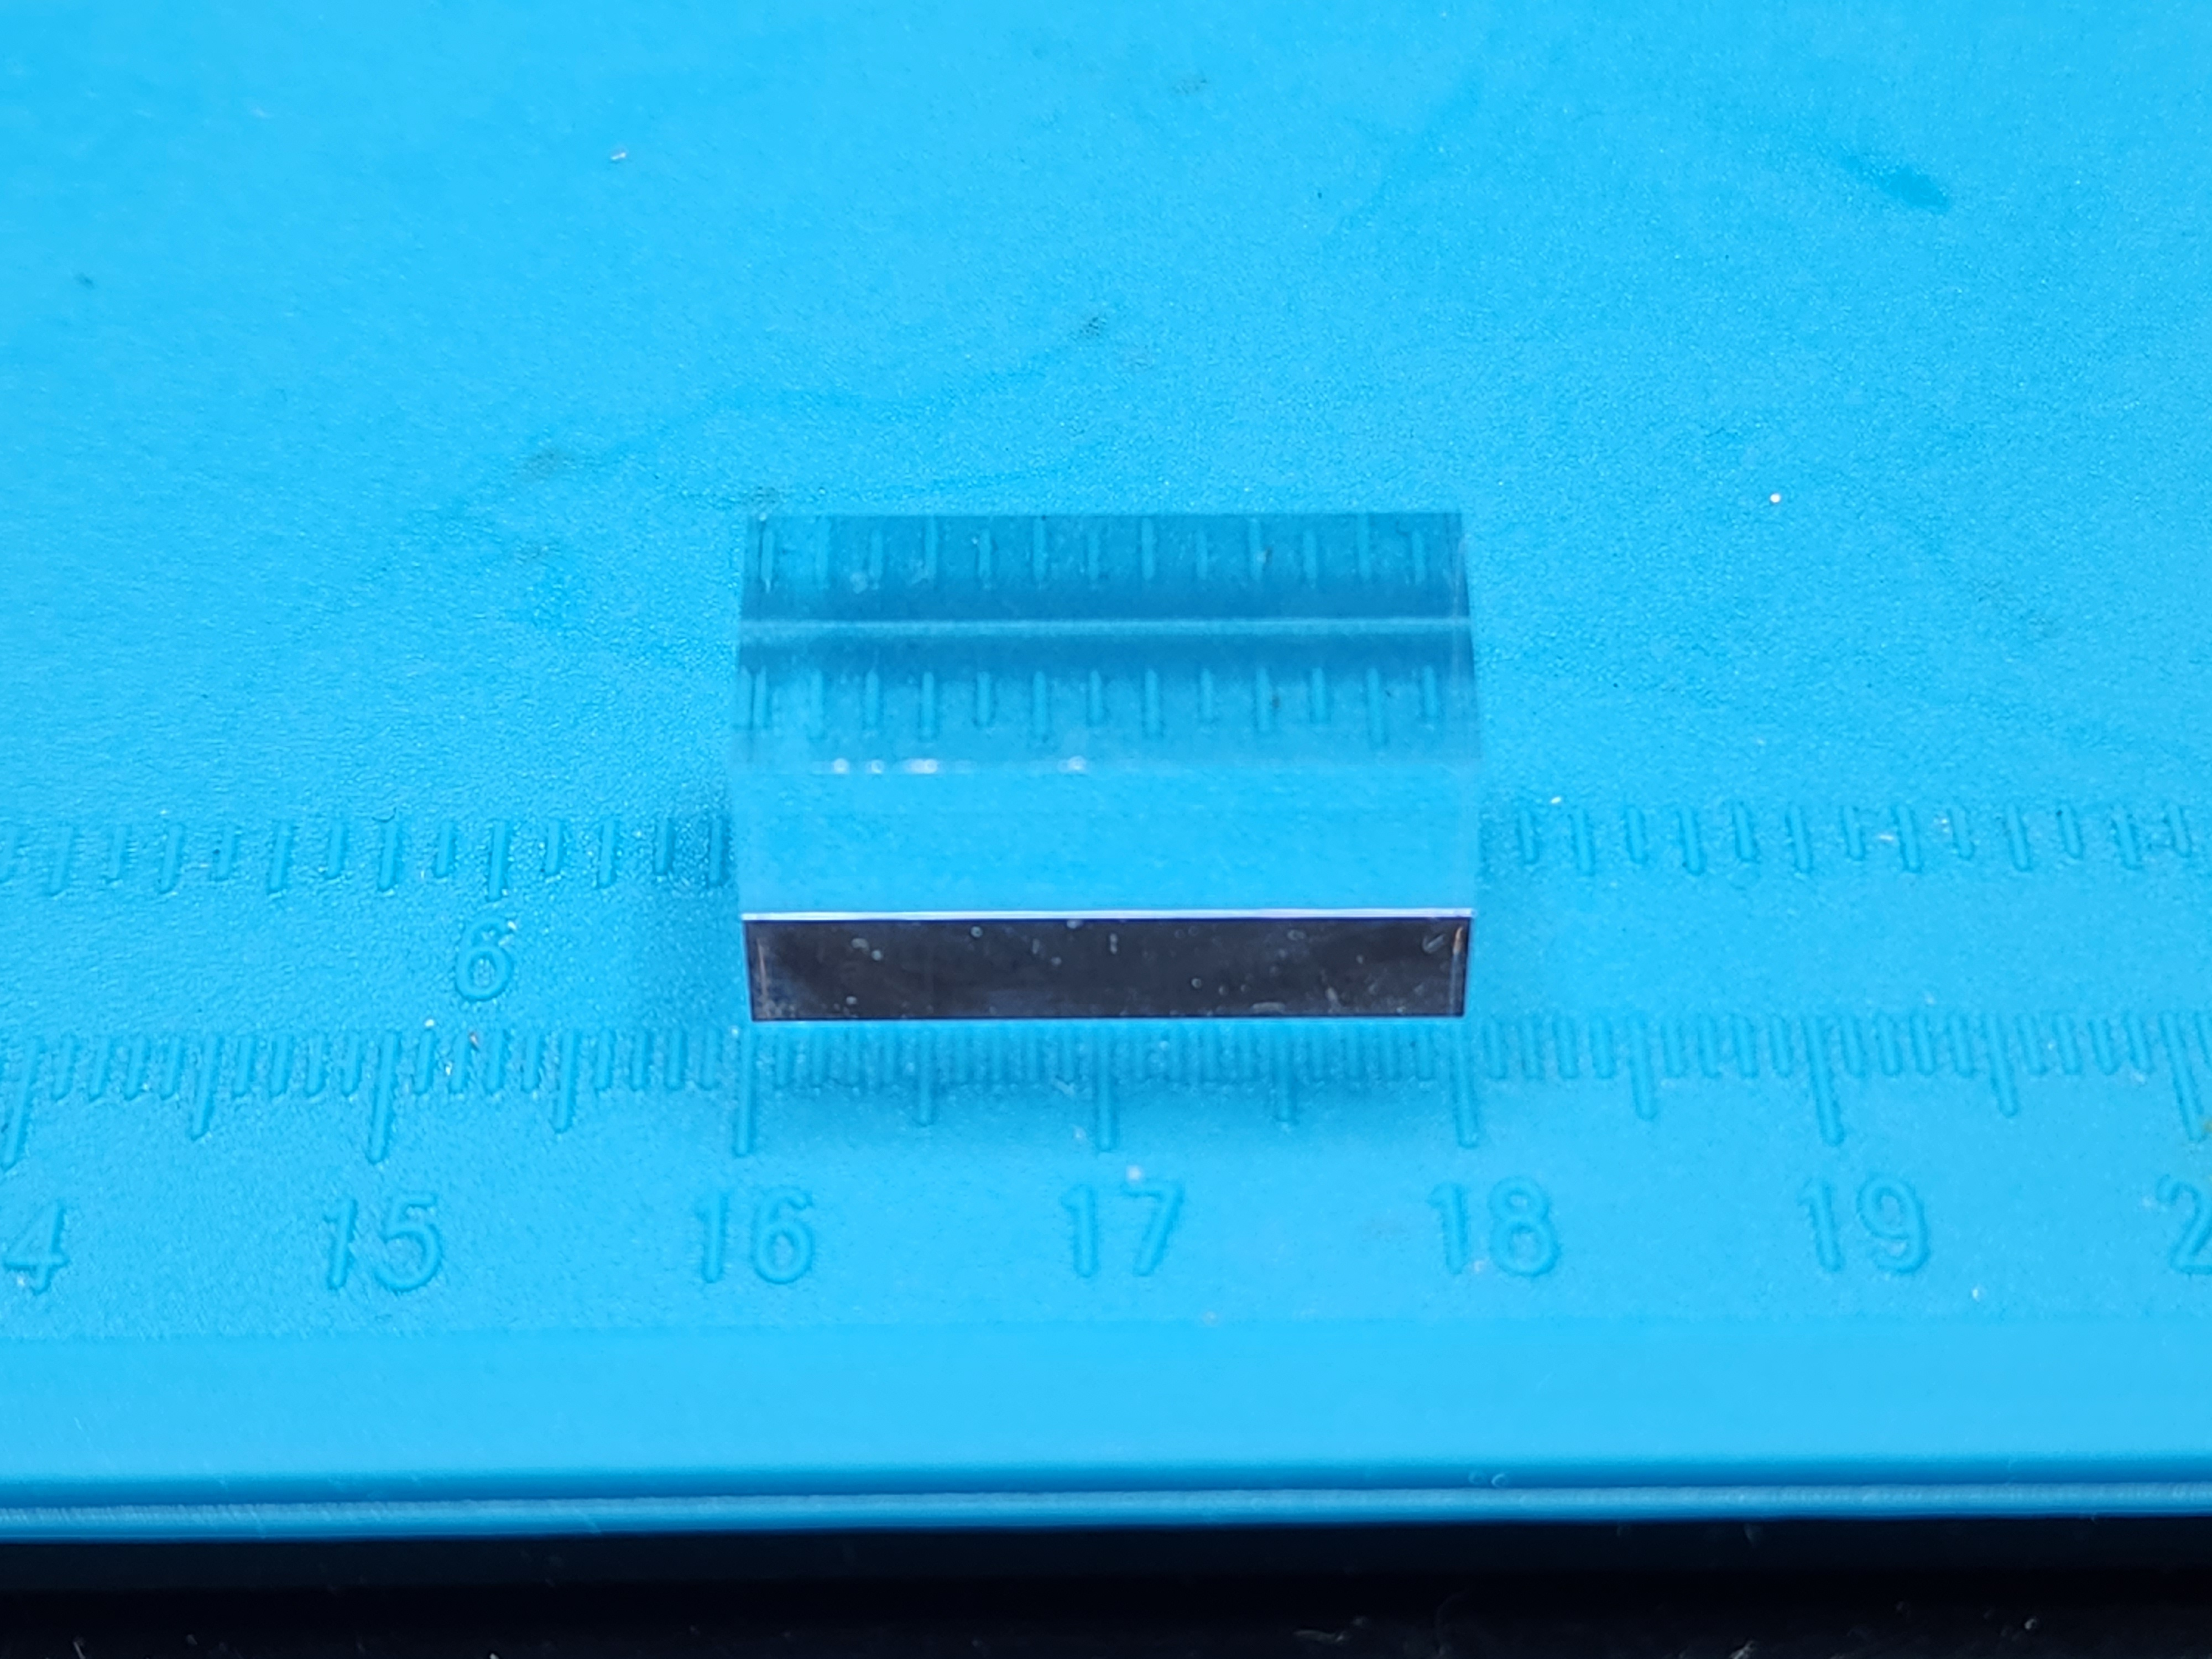
\includegraphics[width=.7\textwidth]{future/LYSO_crystals/LYSO_20_10_10.jpg}
    \end{subfigure}
    \begin{subfigure}[t]{0.49\textwidth}
        \centering
        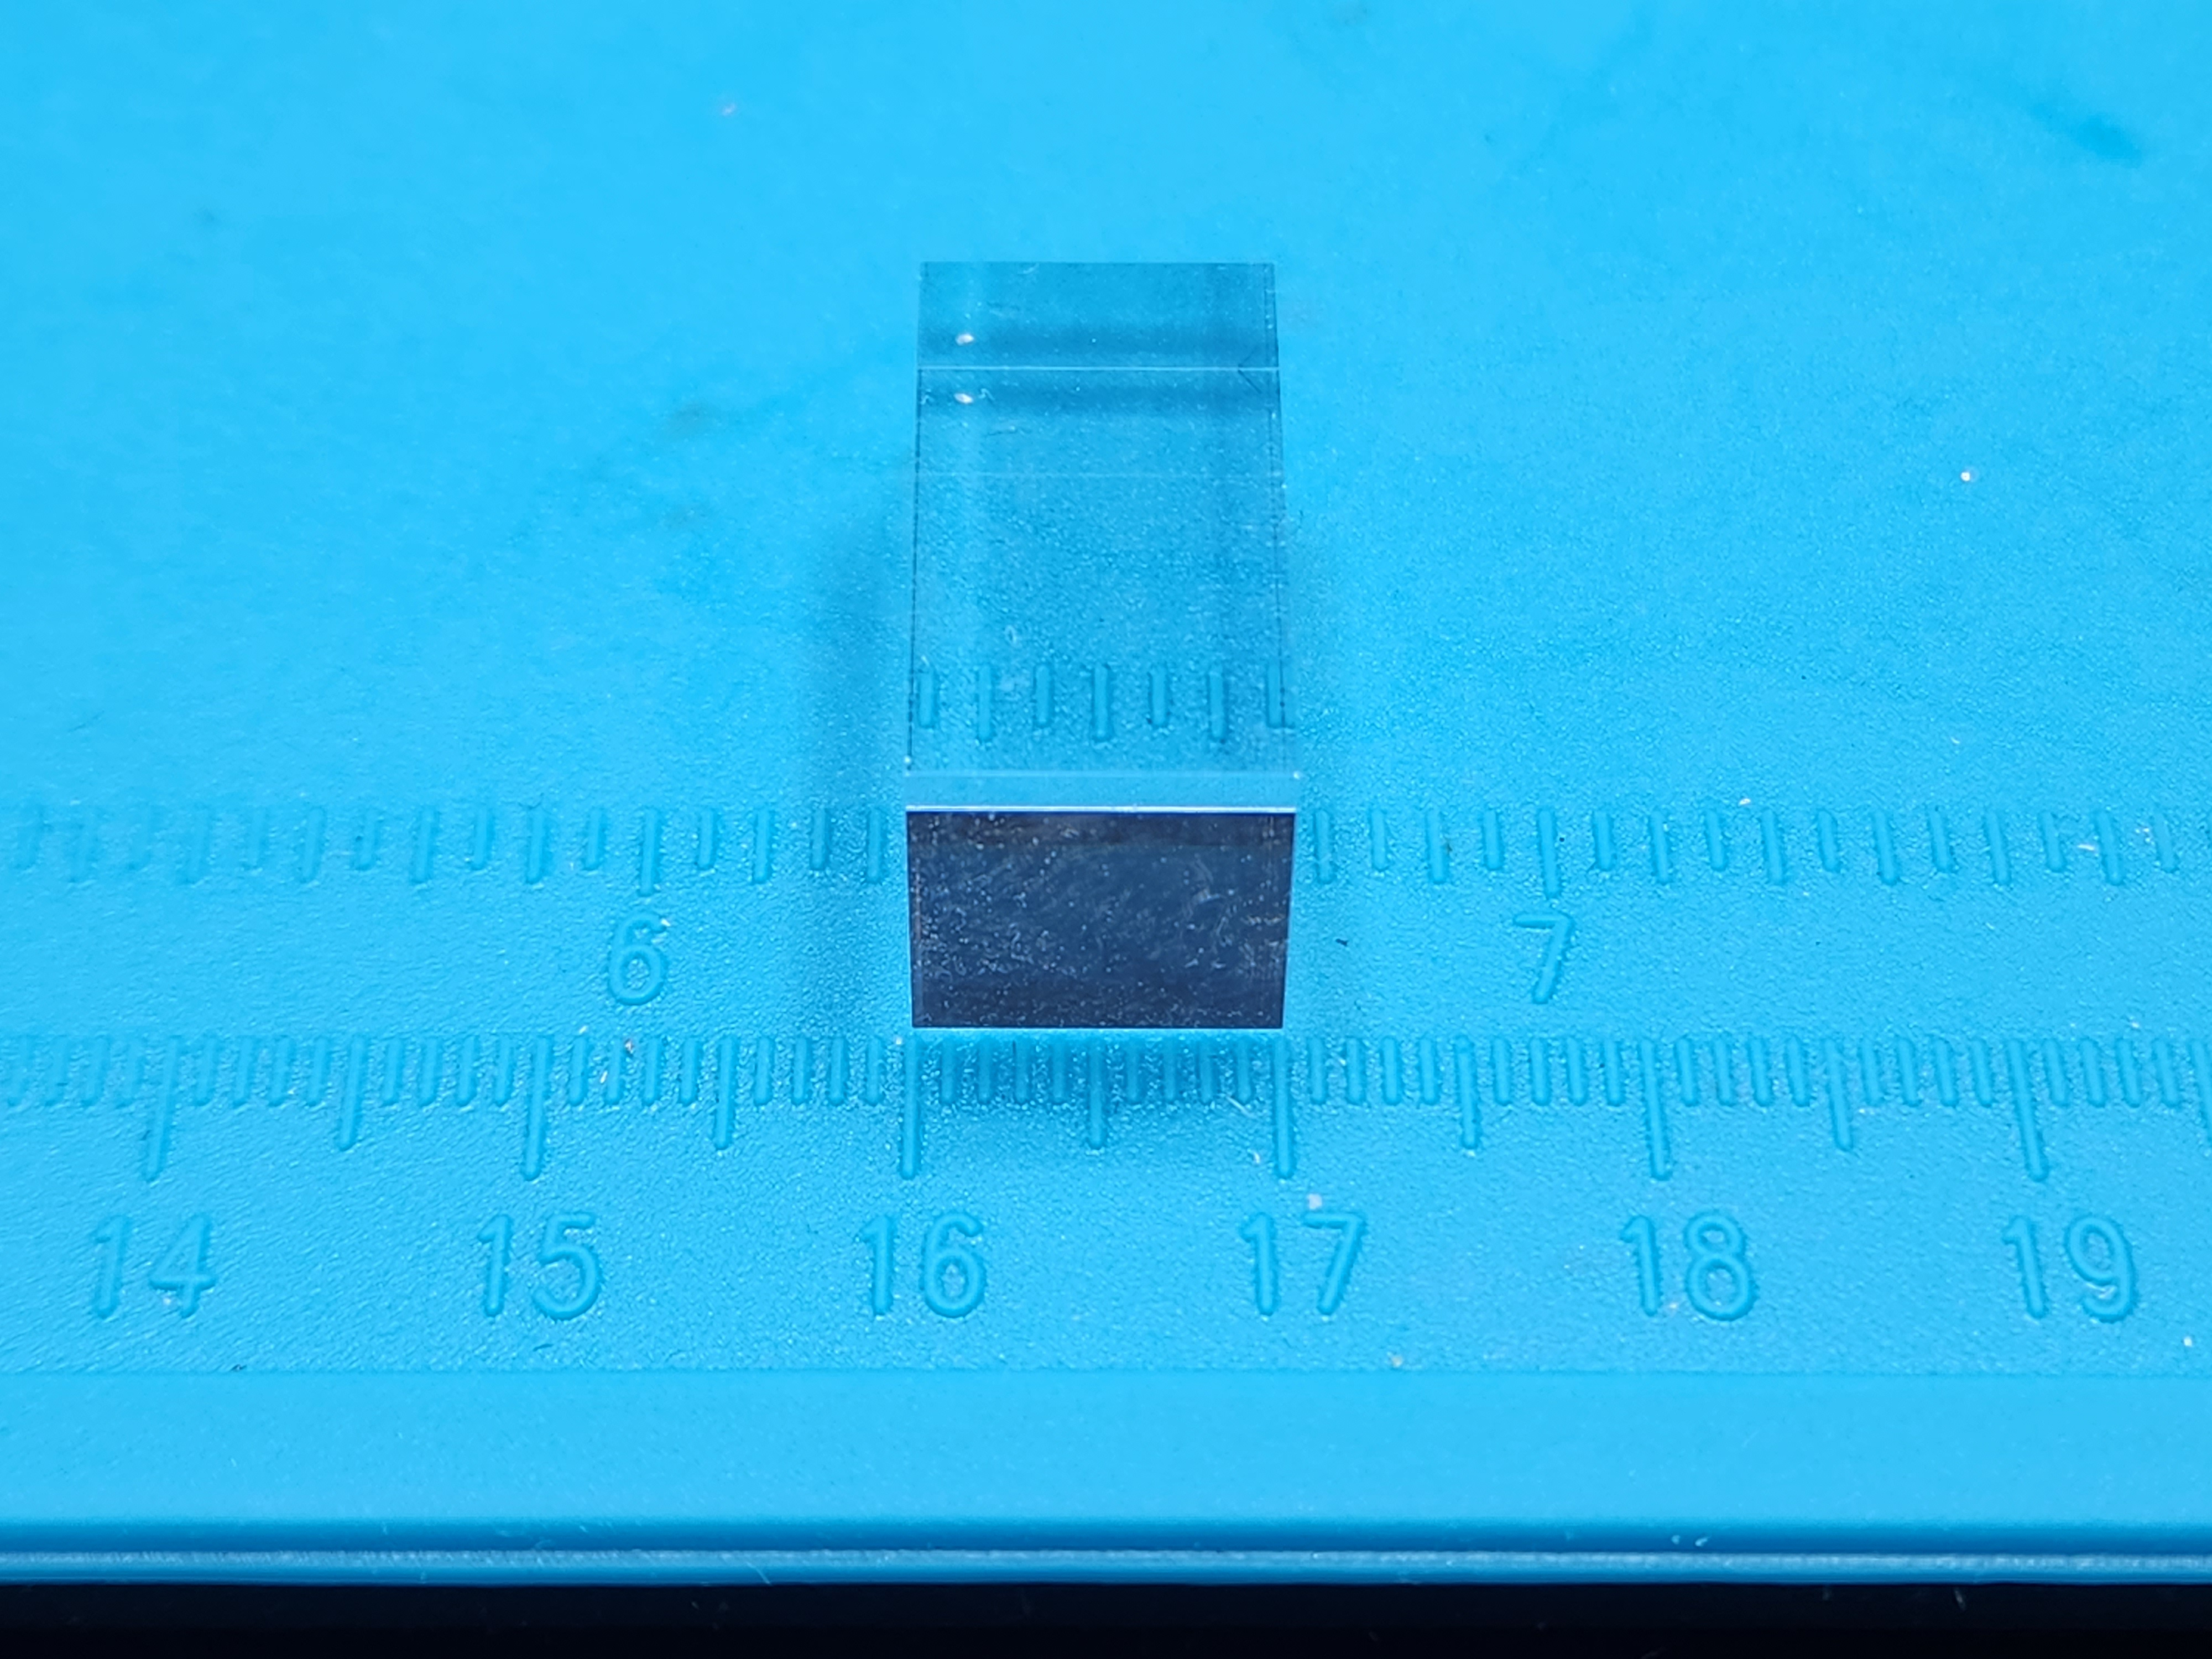
\includegraphics[width=.7\textwidth]{future/LYSO_crystals/LYSO_20_10_10_2.jpg}
    \end{subfigure}
    \medskip
    \begin{subfigure}[t]{\textwidth}
        \centering
        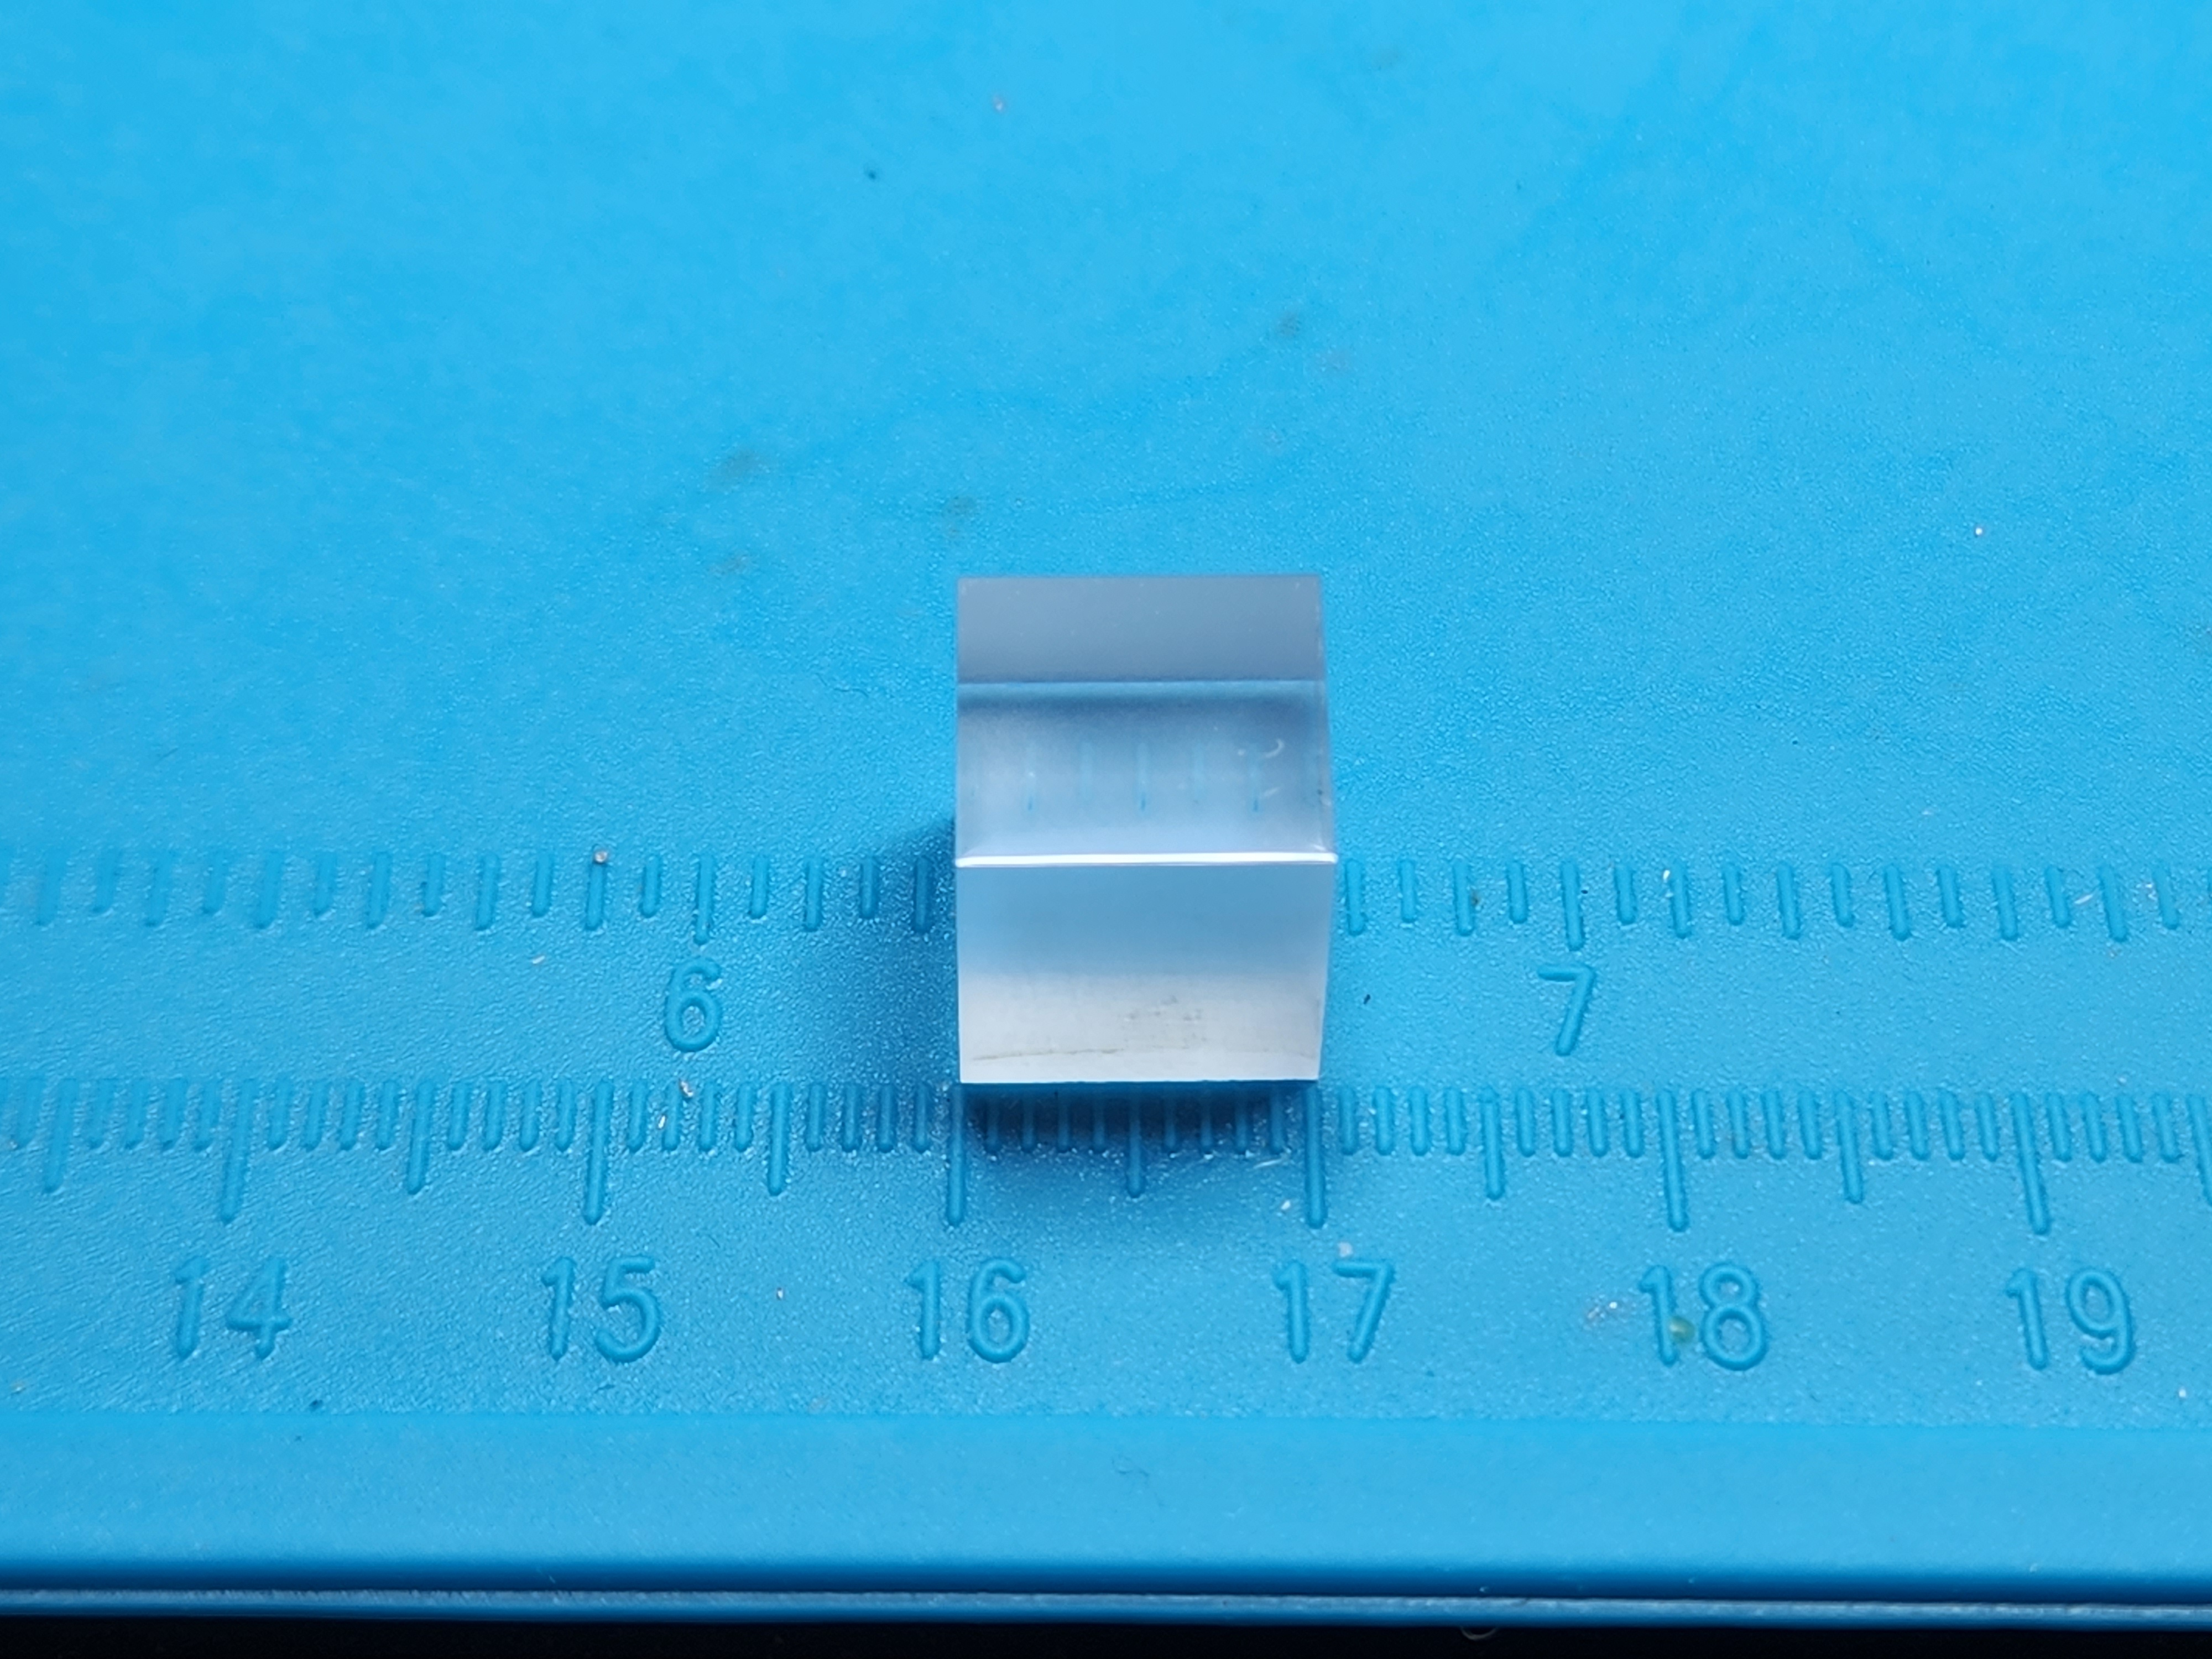
\includegraphics[width=.35\textwidth]{future/LYSO_crystals/LYSO_10_10_10.jpg}
    \end{subfigure}
    \caption{\label{fig:LYSO_crystals}Dimensions of LYSO crystals used to test the CosmicWatch response.}
\end{figure}

The scintillator size can have great consequences on the resulting spectra and therefore energy resolution, as is showcased in subsections \ref{sec:simulated_spectra} and \ref{sec:collected_produced}, this opens up a great opportunity to explore the possibility of testing other crystal sizes, since up until now only the $4\times4\times22$ \unit{\mm\cubed} LYSO has been used to measure spectra. Some photos of available crystal sizes provided by Luxium are shown in Fig. \ref{fig:LYSO_crystals}. On the other hand, it could also be useful to try BGOs, these crystals are also sold for relatively low prices, this however tends to show better results at energy ranges above our use case.